\documentclass[conference,compsoc]{IEEEtran}

\usepackage{etex}

\usepackage[pdftex]{graphicx}
\usepackage{amsmath}
\usepackage{xcolor}
\usepackage{tikz}
\usepackage{schemabloc}
\usepackage{multicol}
\usepackage{amssymb}
\usepackage{enumerate}
\usetikzlibrary{circuits}
\usetikzlibrary{calc}
\usetikzlibrary{shapes,shadows,arrows}
%\usetikzlibrary{positioning}
\usetikzlibrary{topaths}

%------------------------------------> To create hyperlinks
\usepackage[colorlinks=true, linkcolor=black, citecolor=black, urlcolor=blue]{hyperref} %, breaklinks=true

%%------------------------------------> To enrich figures
\usepackage{graphicx}
\usepackage[small]{caption} % for figures legends   
\graphicspath{{./figures/}} % Default path
\usepackage{wrapfig}


%------------------------------------> Setting language
\usepackage[english, brazil]{babel}
\usepackage[utf8]{inputenc}
\usepackage[T1]{fontenc}
\usepackage{subfigure}
\usepackage{enumerate}

%------------------------------------> To enrich code layout 
\usepackage{helvet, courier, type1cm}
\usepackage{listings}                   

%------------------------------------> To enrich figures
\usepackage{graphicx}
\usepackage{epstopdf}
\usepackage{pdfpages}


%------------------------------------> Defining colors
\usepackage{color} 
\definecolor{blackgreen}{rgb}{0,0.4,0}
\definecolor{gray}{gray}{0.3}
\definecolor{blue}{rgb}{0,0,0.5}
\definecolor{green}{rgb}{0,0.5,0}
\definecolor{lightgreen}{rgb}{0,0.6,0}
\definecolor{purple}{rgb}{0.5,0,0.5}
\definecolor{darkred}{rgb}{0.5,0,0}
\definecolor{dkgreen}{rgb}{0,0.6,0}
\definecolor{mauve}{rgb}{0.58,0,0.82}
\definecolor{orange}{rgb}{1,0.5,0}
\definecolor{kugray5}{RGB}{224,224,224}


%------------------------------------> Changing default geometry layout
\usepackage{geometry}
\usepackage{setspace}
\addtolength{\hoffset}{-0.3cm}
\addtolength{\voffset}{-.5cm}
\addtolength{\textheight}{1.5cm}
\addtolength{\textwidth}{0.8cm}

%------------------------------------> To enrich tables
\usepackage{multirow}
\usepackage{colortbl}


%------------------------------------> Using fancy features for header and footpage 
\usepackage{fancyhdr}

%------------------------------------> To create hyperlinks
%\usepackage[colorlinks=true, linkcolor=blue, citecolor=blue, urlcolor=blue] {hyperref}%, breaklinks=true

%% Para usar matlab2tickz
\usepackage{pgfplots}
%% and optionally (as of Pgfplots 1.3):
%\pgfplotsset{compat=newest}
%\pgfplotsset{plot coordinates/math parser=false}
%\RequirePackage[demo]{graphicx} 

% Formating code typeset structure
\lstset{language=MATLAB, %C
%
basicstyle=\ttfamily\scriptsize,        % code font size
keywordstyle=\color{red}\textbf,	% key words style
commentstyle=\color{blue},		% comments style
%
% numbers=left,                   	% where to put line numbers
% numberstyle=\ttfamily\scriptsize, 	% line nuimbers style
% numberblanklines=false,			
%
captionpos=t,                   % put legend under the text
frame=TB,	                 
%
showspaces=false,               % show spaces
showstringspaces=false,         % show characters
showtabs=false,                 % show tabulation with characters
tabsize=4,	                % tabulation size
%
moredelim=[s][\color{blackgreen}]{'}{'},
moredelim=[s][\color{blackgreen}]{"}{"},
}

\usepackage[]{mcode}
\usepackage{tikz}
\usetikzlibrary{shapes,arrows}
\usetikzlibrary{calc}
\usepackage{verbatim}


\ifCLASSOPTIONcompsoc
  \usepackage[nocompress]{cite}
\else
  \usepackage{cite}
\fi

\begin{document}

\title{Métodos Estocásticos para Minimização Vetorial\\ CPE-737 Otimização}


\author{\IEEEauthorblockN{Arthur Fernandes S. Xaud}
\IEEEauthorblockA{Eng. Controle e Automação\\
PEE-COPPE}
\and
\IEEEauthorblockN{Carolina Calvo P. S. Neves}
\IEEEauthorblockA{Eng. Controle e Automação\\
PEE-COPPE}
\and
\IEEEauthorblockN{Gabriel Felippe Pacheco}
\IEEEauthorblockA{Eng. Controle e Automação\\
PEE-COPPE}}


% make the title area
\maketitle

% As a general rule, do not put math, special symbols or citations
% in the abstract
\begin{abstract}
Neste trabalho, para resolução dos problemas de otimização tipicamente abordados em sala de aula, foram implementados dois métodos de natureza estocástica: Simulated Annealing e Estratégias Evolutivas. Ambos foram bem-sucedidos ao serem aplicados a diversas funções objetivo, mas a função Ackley foi a escolhida para a apresentação dos resultados devido a sua natureza multimodal. Tratou-se também o caso de dimensões maiores que dois para testar a capacidade dos algoritmos.\\
\end{abstract}


\IEEEpeerreviewmaketitle


%%%%%%%%%%%%%%%%%%%%%%%%%%%%%%%%%%%%%%%%%%%%%%%%%%%%%%%%%%%%%%%%%%%%%%%%%%%%%%%%
\section{Introdução} % 
\vspace{0.1cm}

A resolução de problemas de otimização pode envolver a utilização de algoritmos determinísticos e estocásticos. Durante muito tempo, os algoritmos determinísticos foram foco principal de estudos devido à sua fundamentação matemática e à garantia de convergência sob determinadas condições. Entretanto, esses algortimos podem ser complexos e em sua grande maioria tem seu escopo limitado a funçoes unimodais.

Por conseguinte, com avanço da capacidade computacional, começaram a surgir alternativas heurísticas, com base ora em idéias mais simples (multiplas avalições da função objetvio) ora na observação da fenômenons naturais. Por essa razão, a implementação desses novos algoritmos é simplificada e as soluções podem ser alcançadas rapidamente, mesmo que com um numero muito superior de iterações se comparado a algortimos determinísticos.

No entanto, como tais metodologias não possuem necessariamente uma fundamentação matemática rigorosa, nem sempre a sua convergência pode ser comprovada, não havendo segurança em certos casos de que uma solução será sempre encontrada. Mesmo sem provas matemáticas, a maior parte dos métodos vêm apresentando resultados surpreendentes ao longo dos anos.

Em geral, os algoritmos heurísticos englobam elementos estocásticos, o que permite a busca do ótimo global evitando os mínimos locais que atrairiam facilmente os algoritmos determinísticos.  Isso ocorre porque o fato de envolverem probabilidades em seu desenvolvimento mune esses algoritmos da possibilidade de seguir em direção a uma região onde a avaliação da função objetivo é mais elevada.

Outro fator importante que impulsionou a utilização dos métodos heurísticos foram os avanços tecnológicos. Atualmente, a capacidade de processamento dos computadores é muito superior àquela existente na época em que os algoritmos determinísticos foram desenvolvidos , permitindo, assim, um número bem maior de avaliações da função objetivo.

Os dois métodos de otimização que serão abordados neste trabalho foram originados a partir das observações de dois processos que ocorrem na natureza, a saber, a evolução de processos termodinâmicos e a evolução das espécies.

O primeiro desses métodos chama-se Simulated Annealing e se baseia no processo de recozimento de metais. Os Algoritmos Genéticos, por sua vez, são aqueles baseados nas teorias de evolucionismo. Ambos são muito poderosos codificando e simulando processos naturais.\\


\section{Simulated Annealing}
\vspace{0.3cm}

O Simulated Annealing, ou Recozimento Simulado, foi proposto por \cite{SA}. O processo físico de \textit{annealing} consiste em aquecer um sólido até uma temperatura $T_0$ acima do seu ponto de fusão. Em seguida, o metal é resfriado lentamente, diminuindo gradativamente sua temperatura até atingir o estado de equilíbrio, de baixa energia, tornando a estrutura do sólido forte, cristalina e livre de imperfeições.

Se esse resfriamento for feito rapidamente, os produtos gerados são pouco estáveis, com maior energia interna, o que poderia ser entendido como uma analogia com pontos locais de energia mínima. Por outro lado, um resfriamento lento faz com que os materiais tenham estruturas mais fortes e estáveis, tendendo para estados com energias ainda menores. Em um longo período de tempo, espera-se que todos os estados tenham sido visitados, permitindo a obtenção do estado de energia mínima, o que poderia ser comparado ao mínimo global de uma função.

O \textit{simulated annealing} utiliza o mesmo conceito desse processo físico. Utilizando o algortimo de 
Metropolis \cite{metropolis}, o método é incializado com uma temperatura inicial $T_0$ elevada que vai decrescendo ao longo do tempo. O decaimento de temperatura proposto originalmente seria regido, em função do tempo, ssspela equação \ref{eq:dec}.

\begin{equation}
T_k = \frac{T_0}{log_2(1+k)}
\label{eq:dec}
\end{equation}

\vspace{0.5cm}

Assim, existem soluções (estados) e custos (energias) até que seja alcançado o equilíbrio naquela temperatura. Uma vez que esse equilíbrio tenha sido atingido, reduz-se a temperatura. O processo é repetido até que a tempertura se aproxime de zero, ou seja, quando o processo está congelado e não há mais diminuição da função custo.

A cada iteração do método em determinada temperatura, um novo estado é gerado a partir do estado corrente aplicando-se uma perturbação gaussiana de tamanho $\varepsilon$. Caso o estado perturbado tenha energia menor que o estado corrente, adota-se o novo estado. Caso contrário, ainda há uma probabilidade de se mudar do estado corrente para o estado perturbado que depende da diferença $\Delta$ de energia entre os dois estados, da temperatura corrente $T_k$ e da constante de Boltzmann $k$, conforme a equação \ref{eq:boltz}.

\begin{equation}
k = e^{-\frac{\Delta}{(kT_k)}}
\label{eq:boltz}
\end{equation}

\vspace{0.3cm}

Vale observar que, quanto maior a temperatura, maior a probabilidade de aceitação de um novo estado, mesmo que isso represente uma deterioração no valor da função objetivo. Em altas temperaturas, cada estado tem praticamente chances iguais de ser o estado corrente. 

Da mesma maneira, quanto menor a temperatura, menor a chance de aceitação do novo estado. Em outras palavras, o estado corrente tende a não se alterar com a diminuição da temperatura. Portanto, em baixas temperaturas, apenas estados com baixa energia irão ter alta probabilidade de se tornarem estados correntes. Dessa forma, enquanto a temperatura diminui, a energia do sistema também diminui e a função custo vai tendendo para um ponto ótimo.

Portanto, com a temperatura tendendo a zero, diminui-se a chance de o algoritmo tomar uma direção de aumento da função objetivo. Então, com o tempo, o algoritmo vai se tornando apenas um método de descida determinístico.\\


\subsection{FSA (Fast Simulated Annealing)}

Apesar de o Simulated Annealing exigir um decaimento lento da temperatura, a evolução da temperatura baseada em $(log_2)^{-1}$ pode ser muito lenta, retardando em excesso o processamento. \\

Para contornar essa limitação, foi proposto em \cite{FSA} uma nova equação para a atualização da temperatura conforme a equação \ref{eq:FSA}.

\begin{equation}
T_k = \frac{T_0}{(1+k)}
\label{eq:FSA}
\end{equation}

\vspace{0.3cm}

É importante lembrar que, embora essa atualização não possua nenhuma prova matemática de convergência, na maioria das vezes, é mais utilizada do que a fórmula original por acelerar muito o desenvolvimento do algoritmo. O fluxograma apresentado na figura \ref{fig:SA_flow}.

\begin{figure}[!h]
\centering
\includegraphics[scale=0.72]{SA.pdf}
\caption{Método Simulated Annealing}
\label{fig:SA_flow}
\end{figure}
   
\section{Algoritmos Genéticos : Estratégias Evolutivas}

As Estratégias Evolutivas são uma das alternativas possíveis em Algoritmos Genéticos. Estes se inspiram na evolução natural para resolver problemas de Otimização através de algoritmos de busca estocástica. 

Desta maneira, consideram a analogia da  aptidão dos indivíduos de uma população como função custo a ser minimizada/maximizada. Assim, cada indivíduo da população representa um ponto no domínio da função objetivo.

Uma população representa, portanto, um conjunto de indivíduos que evoluem ao longo do tempo em consequência de seu cruzamento (recombinação de genes), de mutações e da própria seleção natural, resultando na sobrevivência daqueles mais aptos (melhoress otimizadores da função custo).

Primeiramente, chama-se seleção de pais o processo através do qual se define quais indivíduos da população gerarão filhos, sendo possível que a população inteira seja considerada para tal fim. Em outras palavras, antes da recombinação de indivíduos, há a determinação de quais elementos farão parte desta etapa. O cruzamento em si corresponde à geração de novos elementos com características herdadas de ambos os pais. 

Em seguida, perturbações aleatórias são aplicadas aos indivíduos da população, ao que se dá o nome de mutações. E, finalmente, em meio à população anterior e filhos gerados, a seleção de sobreviventes consiste no processo de determinação dos indivíduos que seguirão até a geração seguinte.

Dessa maneira, à medida que as gerações evoluem, espera-se que a população mude, de maneira que se encaminhe cada vez mais concentrada em direção ao mínimo da função objetivo, já que a tendência da seleção natural é a de que os mais aptos sobrevivam.

Entretanto, os fatores aleatórios envolvidos com tais fenômenos podem levar algumas vezes à perda de características desejáveis da população (deriva genética). 

Particularmente, a representação de um típico ES é contínua, a seleção de pais é aleatória e uniforme e as mutações são em forma de perturbação gaussiana.
 
A seleção de sobreviventes, por sua vez, é determinística, ou seja, os mais aptos sobrevivem em contraposição ao caso estocástico, no qual um indivíduo menos apto pode permanecer na população, apesar de sua baixa probabilidade de sobrevivência.

O diferencial das estratégias evolutivas reside sobretudo no fato de serem capazes de se adaptar no sentido de encontrar tamanhos de perturbações adequadas para obtenção de bons resultados \cite{notas_aula_JG} dependo da situação atual da população como um todo e de cada indivíduo separadamente. 

Desse modo, um indivíduo é perturbado pela adição, a cada uma de suas dimensões, de um número aleatório resultante de uma distribuição normal com média zero e desvio padrão unitário.

Além disso, o princípio da auto-adaptação se baseia na regra de \textit{Rechenberg}, segundo a qual a taxa de sucesso das mutações deve ser de 0.2. Nesse sentido, uma mutação é considerada bem-sucedida quando o indivíduo resultante da mutação possui uma aptidão mais elevada que a do indivíduo original.

Dessa forma, se a taxa de sucesso das mutações for inferior a esse valor, aumenta-se o desvio padrão $\sigma$ da distribuição que provoca a mutação, de maneira a considerar um espaço de busca maior e evitar uma convergência prematura. Por outro lado, se as mutações estiverem sendo consideradas ineficientes, diminui-se o espaço de busca. Sendo assim, conforme a função se aproxima do mínimo, há redução do tamanho dos passos.

Portanto, é interessante mencionar que o tamanho do passo de mutação é alterado de acordo com um \textit{feedback} do processo evolucionário.

\subsection{Representação de Indivíduos}

No algoritmo implementado, foram escolhidas mutações não correlacionadas e diferentes tamanhos de passos para cada dimensão do problema ($n_\sigma=n$), já que a inclinação de uma função a ser minimizada pode ser diferente em cada direção.

Assim, um elemento populacional é descrito não somente pelas variáveis do problema ($x_i$), mas também pelos seus parâmetros de estratégia (parâmetros do operador de mutação), como na equação \ref{eq:represent}:

\begin{equation}
(x_1, ... , x_n,\sigma_1, ... , \sigma_n) %\alpha_1, ... , \alpha_{n_\alpha})
\label{eq:represent}
\end{equation}


 \subsection{Inicialização da População}
 
 A população de $\mu$ indivíduos foi inicializada ao redor de $x_0$, conforme a equação \ref{eq:init}, onde $n$ corresponde à dimensão do problema.\\
 
 \begin{equation}
 x_k = x_0 \, e^{\frac{N(0,1)}{\sqrt{n}}}, \hspace{0.2cm} para \, k=1,...\mu
 \label{eq:init}
 \end{equation}
  
 \subsection{Recombinação}
    
Considerou-se a recombinação discreta nas variáveis do problema e intermediária nos parâmetros de estratégia. Isso significa que, para as variáveis de dimensão do problema, escolhe-se para o filho aleatoriamente o valor de $x_i \,(para \, i=1,...n)$ de um dos pais. No caso dos parâmetros de estratégia do filho gerado, considerou-se a média aritmética das estratégias dos pais. \\

 \subsection{Mutação}
  
A particularidade interessante da auto-adaptação está relacionada à representação: como os parâmetros de estratégia são parte do indivíduo, eles também sofrem variação e seleção.  Assim, primeiro modifica-se o valor de $\sigma$ para depois aplicar a mutação a $x_i$ com o novo desvio padrão $\sigma'$, conforme as equações:

 \begin{eqnarray}
 \sigma'_i &= &\sigma_i \, e^{\tau_1  \, N(0,1)} \,  e^{\tau_2  \, N_i(0,1)} \\ \nonumber
 x_i'&=& x_i + \sigma'_i \, N_i(0,1)
 \end{eqnarray}
 \vspace{-0.4cm}

\begin{flushleft}
Onde
\end{flushleft}	
\vspace{-0.3cm}	

\begin{eqnarray}
 \tau_1 &=& \frac{\alpha_1}{\sqrt{2\,n}}    \nonumber \\ 
 \tau_2 &=& \frac{\alpha_2}{\sqrt{2\sqrt{n}}} %\\
\end{eqnarray}

 \vspace{0.3cm} 
Dessa maneira, os pontos no espaço de busca onde o indivíduo tem determinada probabilidade de ser posicionado formam uma elipse ao redor do indivíduo original.
 
 \subsection{Seleção de Sobreviventes}
 
 No presente algoritmo a seleção dos sobreviventes foi realizada deterministicamente através de ranqueamento da aptidão (avaliação da função objetivo) dos filhos gerados, sem sorteio. A seleção baseada apenas na prole é uma estratégia que ajuda a escapar de mínimos locais, já que descarta soluções antigas.
 
O número de indivíduos sobreviventes corresponderá sempre ao tamanho original da população, eliminando filhos menos aptos se $\lambda>\mu$. Uma proporção de aproximadamente $\lambda=7\mu$ implica em pressão seletiva alta. 

A auto-adaptação do algoritmo implica que um sobrevivente representa não somente bons minimizadores $x_i$ do problema (o que se traduz em aptidão elevada), mas também bons valores de estratégia, já que os $\sigma'_i$ se provaram eficientes na geração de $x_i'$ a partir de $x_i$.
   
\subsection{Critério de Parada}

O critério de parada escolhido, evidenciado no fluxograma de implementação do algoritmo apresentado na figura \ref{fig:ES_flow}, considera o quanto a média da aptidão da população variou de uma geração para a outra, baseado na consideração em conjunto de dois limites mínimos: um absoluto e outro relativo.

Caso a função objetivo varie menos do que esses limiares, considera-se que o algoritmo está suficientemente perto do mínimo da função. Caso o limiar não seja atingido, o processo continua até que um numero maximo predefinido de avaliações da função custo.

\begin{figure}[!hctb]
\centering
\scalebox{0.74}{\input{ES.tex}}
\caption{Método de Estratégias Evolutivas}
\label{fig:ES_flow}
\end{figure}
   

\section{Resultados}

Apresentaremos neste relatório o resultado da aplicação dos referidos métodos à função Ackley da equação \ref{eq:ackley} inicialmente com duas dimensões (i=2), sabendo que seu minimo global encontra-se em $f(\textbf{x}^*)=0$ para $\textbf{x}=\textbf{0}$.

 \begin{equation}
 \begin{split}
f(\textbf{x}) =  -20\, & exp\left (-0.2 \sqrt{\frac{1}{n} \sum_{i=1}^n x_i^2} \right) -\\
		              & exp \left( \frac{1}{n} \sum_{i=1}^n cos(2\pi x_i) \right) + 20 + e
 \label{eq:ackley}
 \end{split}
 \end{equation} 
 
 \subsection{Simulated Annealing}

Para aplicação do Simulated Annealing à função Ackley, utilizou-se um número de rodadas por temperatura de $N=500$ e um número $K=100$ de temperaturas. Isso garante um máximo de $50000$ iterações para a busca do mínimo da função.

Foi utilizada uma temperatura inicial alta de $T_0=5$, garantindo que o algoritmo seja inicializado com probabilidades praticamente equivalentes para os estados em volta do ponto inicial.

O tamanho de perturbação utilizado também foi alto, $\varepsilon=0.1$, o que garante uma região de exploração maior, porém dificulta o ajuste fino para a obtenção do ponto mínimo.Ao algoritmo foi adicionado um fator extra de taxa de sucesso $s=0.5$ que muda de temperatura caso o número de aceitações de novos pontos em uma mesma temperatura ultrapasse o número $N*s$. 

Essa medida torna o algoritmo mais rápido durante a busca inicial aleatória. Por último, foi utilizado o método FSA para evolução da temperatura com o tempo.

Os resultados correspondentes aparecem nas figuras \ref{fig:SA_ackley_3D}, \ref{fig:SA_ackley_T}, \ref{fig:SA_ackley_curvNivel} e \ref{fig:SA_ackley_P}. Tambem são apresentados os resultados nas tabelas \ref{tab:SA_ackley} e \ref{tab:min_SA}.

\begin{figure}[!hctb]
\centering
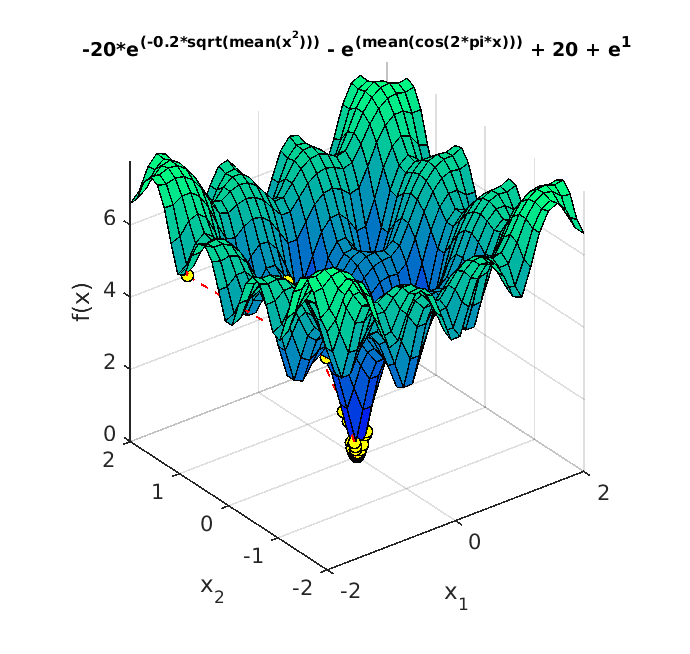
\includegraphics[scale=0.65]{SA_ackley_3D.eps}
\caption{Função Ackley minimizada com Simulated Annealing}
\label{fig:SA_ackley_3D}
\end{figure}

\begin{figure}[!hctb]
\centering
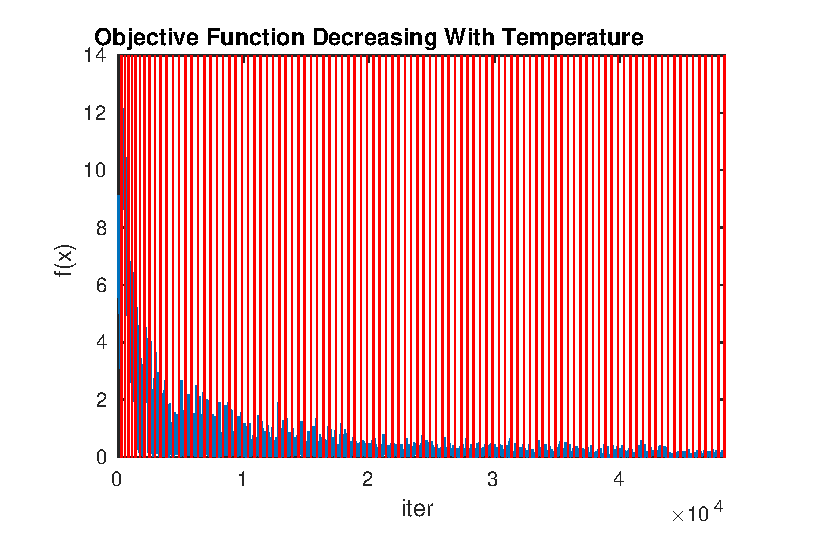
\includegraphics[scale=0.65]{SA_ackley_T.eps}
\caption{Evolução da Função Ackley no tempo separadas por temperaturas}
\label{fig:SA_ackley_T}
\end{figure}

\begin{figure}[!htcb]
\centering
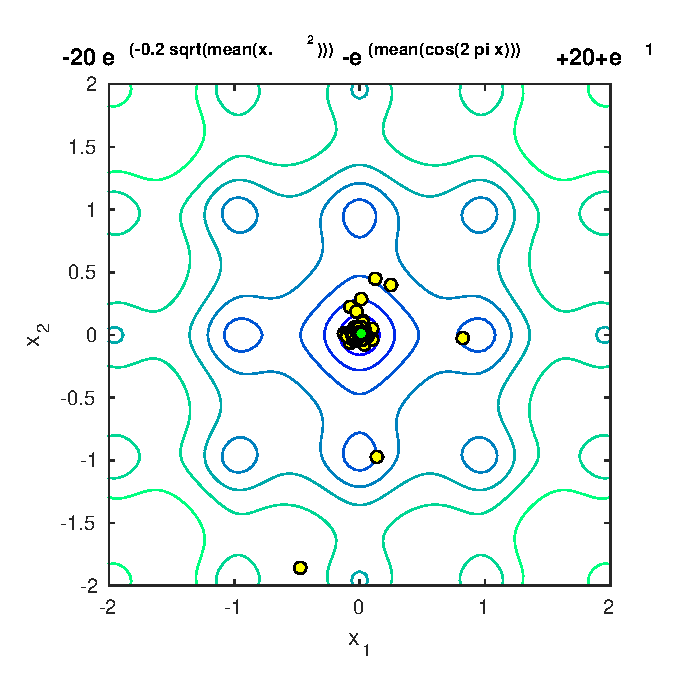
\includegraphics[scale=0.65]{SA_ackley_curvNivel.eps}
\caption{Função Ackley minimizada com Simulated Annealing - Curvas de Nível}
\label{fig:SA_ackley_curvNivel}
\end{figure}

\begin{table}[!htcb]
  \centering
  \begin{tabular}{|c|c|c|c|c|}
    \hline
    \rowcolor{kugray5}
		    &     $x(1)$   &       $x(2)$   &    $f(x)$    & T \\ \hline
\cellcolor{kugray5}1	  &   -3.6573   &  -1.3597	  &   10.6476   &  	5 \\ \hline
\rowcolor{kugray5}10	  &   0.0119	  &   0.0154	  &   0.0650	   &  4.545455e-01     \\ \hline
\cellcolor{kugray5}20	  &   0.0232	  &   0.1169	  &   0.6759	   &  2.380952e-01     \\ \hline
\rowcolor{kugray5}30	  &   0.0485	  &   -0.0160	  &   0.2124	   &  1.612903e-01     \\ \hline
\cellcolor{kugray5}40	  &   0.0133	  &    0.0563	  &   0.2502	   &  1.219512e-01     \\ \hline
\rowcolor{kugray5}50	  &   -0.0214   &  	0.0016	  &   0.0729	   &  9.803922e-02     \\ \hline
\cellcolor{kugray5}60	  &   0.0106	  &    0.0098	  &   0.0464	   &  8.196721e-02     \\ \hline
\rowcolor{kugray5}70	  &   -0.0339   &  	-0.0404	  &   0.2216	   &  7.042254e-02     \\ \hline
\cellcolor{kugray5}80	  &   0.0433	  &    0.0004	  &   0.1715	   &  6.172840e-02     \\ \hline
\rowcolor{kugray5}90	  &   -0.0216   &  	0.0208	  &   0.1085	   &  5.494505e-02     \\ \hline
\cellcolor{kugray5}100	  &   0.0096	  &    0.0136	  &   0.0544	   &  5.000000e-02     \\ \hline
	\end{tabular}
  \caption{Tabela com os estados e a energia no final de cada temperatura}
  \label{tab:SA_ackley}
\end{table}

As figuras  \ref{fig:SA_ackley_3D}, \ref{fig:SA_ackley_T} e \ref{fig:SA_ackley_curvNivel} apresentam a energia dos estados ao final de cada temperatura, conforme a tabela \ref{tab:SA_ackley}. 

Observa-se que a energia decresce com a diminuição da temperatura como era esperado. É possível observar também que, em determinados pontos, a energia aumenta mesmo com a temperatura diminuindo. Esse é o principal efeito desse método, a capacidade de ter alguma probabilidade de aumentar o valor da função objetivo, o que é necessário para escapar de mínimos locais.

\begin{table}[!htcb]
  \centering
  \begin{tabular}{|c|c|c|c|}
    \hline
    \rowcolor{kugray5}     $x(1)$   &    $x(2)$   &    $f(x)$    &   iter \\ \hline
		  				   0.0004	&    0.0007	  &    0.0023	 &   48360 \\ \hline
	\end{tabular}
  \caption{Estado mínimo e energia encontrados pelo SA}
  \label{tab:min_SA}
\end{table}

Como visto na tabela \ref{tab:min_SA}, o minimizador foi assumido como estando em $x= \begin{bmatrix}0.0004&0.0007\end{bmatrix}^T$, onde a função vale 0.0023. Optou-se por utilizar o mínimo correspondente ao estado visitado durante o resfriamento com menor energia. É possível observar que o método realmente está encontrando um valor próximo do mínimo. Executando o algoritmo por mais tempo, ou seja, aumentando o número de temperaturas, espera-se encontrar um resultado ainda mais próximo no mínimo.

\begin{figure}[!htcb]
\centering
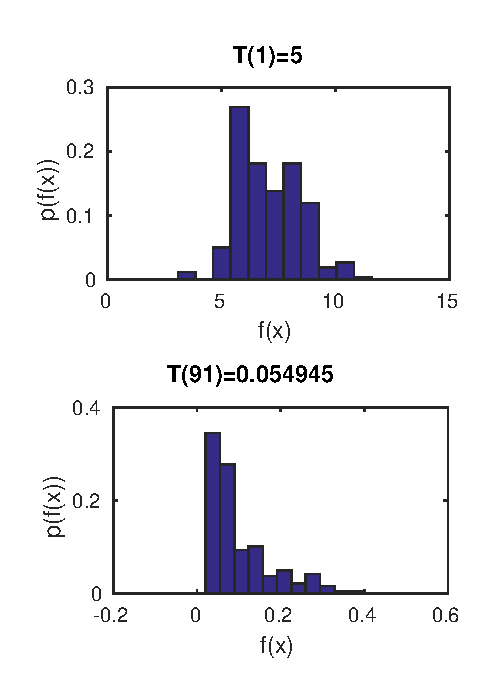
\includegraphics[scale=0.80]{SA_ackley_P.eps}
\caption{Probabilidade do estado corrente possuir energia entre intervalos para determinadas temperaturas}
\label{fig:SA_ackley_P}
\end{figure}

Testou-se também a aplicação do algoritmo à mesma função Ackley com três dimensões. Os parâmetros foram mantidos os mesmos do caso com duas dimensões, porém agora o ponto inicial é $x_0= \begin{bmatrix}-2& 1& 3\end{bmatrix}$. 

\begin{figure}[!htcb]
\centering
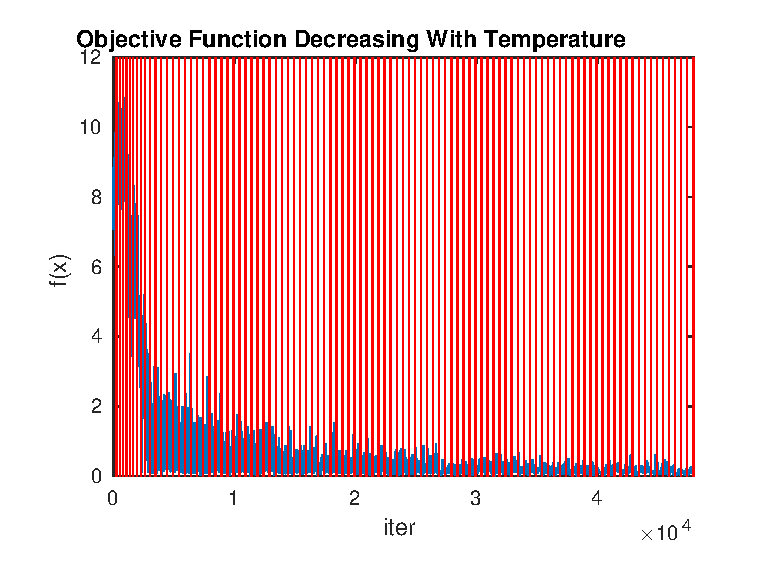
\includegraphics[scale=0.65]{SA_ackley_T_3dim.eps}
\caption{Evolução da Função Ackley no tempo separadas por temperaturas - caso 3 dimensões}
\label{fig:SA_ackley_T_3dim}
\end{figure}


\begin{table}[!htcb]
  \centering
  \begin{tabular}{|c|c|c|c|c|}
    \hline
\rowcolor{kugray5}           &     $x(1)$   &       $x(2)$   &   $x(3)$     &     $f(x)$    \\ \hline
\cellcolor{kugray5}1	  &    2.3139	&     4.0097	 &    1.5893	  &    1.0429e+1	\\ \hline
\rowcolor{kugray5}10	  &    0.0414	&     -0.0547	 &    0.1126	  &    5.8691e-1	\\ \hline
\cellcolor{kugray5}20	  &   -0.0409	&     0.0838	 &    -0.0649	  &    4.7809e-1	\\ \hline
\rowcolor{kugray5}30	  &   -0.0785	&     0.0162	 &    -0.0267	  &    3.1681e-1	\\ \hline
\cellcolor{kugray5}40	  &    0.0057	&     0.0007	 &    0.0014	  &    1.4282e-2	\\ \hline
\rowcolor{kugray5}50	  &    0.0034	&     -0.0119	 &    0.0014	  &    3.1605e-2	\\ \hline
\cellcolor{kugray5}60	  &   -0.0365	&     -0.0346	 &    -0.0223	  &    1.8003e-1	\\ \hline
\rowcolor{kugray5}70	  &   -0.0038	&     0.0220	 &    -0.0538	  &    1.9344e-1	\\ \hline
\cellcolor{kugray5}80	  &   -0.0248	&     0.0134	 &    0.0268	  &    1.1640e-1	\\ \hline
\rowcolor{kugray5}90	  &   -0.0079	&     -0.0139	 &    0.0122	  &    5.3625e-2	\\ \hline
\cellcolor{kugray5}100   &   -0.0174	&     -0.0009	 &    -0.0057	  &    4.8203e-2	\\ \hline
	\end{tabular}
  \caption{Tabela com os estados e a energia no final de cada temperatura - 3 dimensões}
  \label{tab:SA_ackley_3dim}
\end{table}

A figura \ref{fig:SA_ackley_T_3dim} mostra graficamente o resultado da tabela \ref{tab:SA_ackley_3dim}, apresentando o valor da função objetivo avaliada ao longo do tempo, separada por intervalos de temperatura.

\begin{table}[!htcb]

  \centering
  \begin{tabular}{|c|c|c|c|c|}
    \hline
    \rowcolor{kugray5}     $x(1)$   &    $x(2)$   &   $x(3)$   &   $f(x)$    &   iter \\ \hline
							0.0057   &   	0.0007	   &   0.0014	   &   1.4282e-2   &   	47907\\ \hline
	\end{tabular}
  \caption{Estado mínimo e energia encontrados pelo SA - 3 dimensões}
  \label{tab:min_SA_3dim}
\end{table}

Como visto na tabela \ref{tab:min_SA_3dim}, o minimizador indicado pelo algoritmo nesse caso foi $x= \begin{bmatrix}0.0057&0.0007&0.0014\end{bmatrix}^T$, ponto cuja avaliação da função foi $1.428242e-02$. Optou-se por utilizar novamente o mínimo correspondente ao estado visitado durante o resfriamento com menor energia.

Como esperado, o método realmente está encontrando um valor próximo do mínimo. Executando o algoritmo por mais tempo, ou seja, aumentando o número de temperaturas, espera-se encontrar um resultado ainda mais próximo do mínimo.

\begin{figure}[!htcb]
\centering
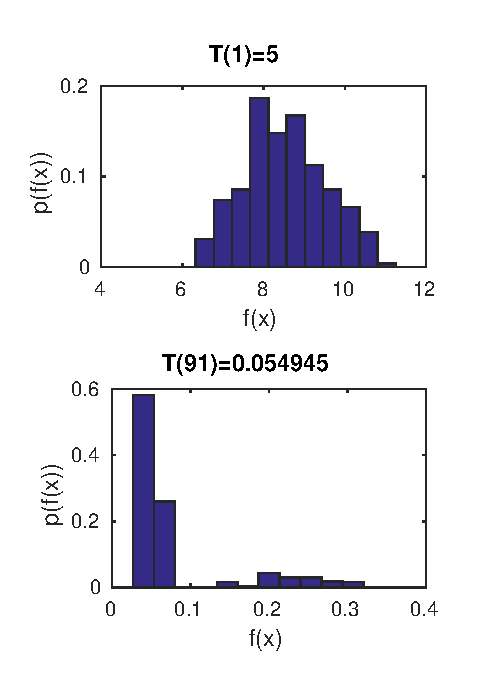
\includegraphics[scale=0.80]{SA_ackley_P_3dim.eps}
\caption{Probabilidade do estado corrente possuir energia entre intervalos para determinadas temperaturas}
\label{fig:SA_ackley_P_3dim}
\end{figure}


\subsection{Estratégias Evolutivas}

Para aplicação do ES à função Ackley, utilizou-se uma população de tamanho $\mu=50$ e $\lambda=250$ para o número de filhos, de maneira a garantir uma boa pressão seletiva e facilitar a convergência. 

As tolerâncias absoluta e relativa para o critério de parada foram respectivamente $\varepsilon_a=10^{-9}$ e $\varepsilon_r=10^{-10}$. Além disso, os parâmetros de perturbação foram $\varepsilon=10^{-2}$, $\alpha_1=\alpha_2=1$. Finalmente, a população foi inicializada aleatoriamente ao redor do ponto $x_0 = \begin{bmatrix}-2 &1\end{bmatrix}^T.$

Os resultados correspondentes aparecem nas figuras \ref{fig:ES_ackley_3D},\ref{fig:ES_ackley_f}, \ref{fig:table} e \ref{fig:ES_ackley_curvNivel}. As figuras  \ref{fig:ES_ackley_3D} e \ref{fig:ES_ackley_f} apresentam o comportamento do indivíduo mais apto da população (mais próximo do mínimo global) em cada geração, conforme a tabela da figura \ref{fig:table}. 

\begin{figure}[!htcb]
\centering
\includegraphics[scale=0.55]{ES_ackley_3D.eps}
\caption{Função Ackley minimizada com Estratégias Evolutivas - Melhor Indivíduo de cada geração}
\label{fig:ES_ackley_3D}
\end{figure}

\begin{figure}[!htcb]
\centering
\includegraphics[scale=0.45]{ES_ackley_f.eps}
\caption{Evolução da Função Ackley avaliada para o melhor indivíduo da população em cada geração}
\label{fig:ES_ackley_f}
\end{figure}

O minimizador foi assumido como estando em $x= \begin{bmatrix}0.0102&0.0065\end{bmatrix}^T$, onde a função vale 0.0382. Este mínimo é considerado por corresponder ao melhor indivíduo da última  (quinta) geração calculada pelo algoritmo com a precisão requerida pelo critério de parada estabelecido.

\begin{table}[!htcb]
  \centering
  \begin{tabular}{|c|c|c|c|}
    \hline
    \rowcolor{kugray5}
		    &     $x(1)$   &       $x(2)$   &    $f(x)$     \\ \hline
	\cellcolor{kugray5}1   &    -0.3944   &   	   0.4201	&    3.8485     \\ \hline
    \rowcolor{kugray5}
		2   &    -0.6040   &       0.0203	&    3.2526     \\ \hline
	\cellcolor{kugray5}3   &    -0.2648   &      -0.0385	&    1.9098     \\ \hline
    \rowcolor{kugray5}
	 	4  &    0.0663	   &      0.0172	&    0.3142     \\ \hline
    \cellcolor{kugray5}5   &    -0.0362   &     -0.0244	&    0.1735     \\ \hline
    \rowcolor{kugray5}
		6   &    0.0102	   &      0.0065	&    0.0382     \\ \hline  
		\end{tabular}
  \caption{Tabela com os melhores indivíduos de cada geração e o valor da função objetivo avaliada}
  \label{fig:table}
\end{table}

A figura \ref{fig:ES_ackley_curvNivel}, por sua vez, evidencia a população inteira de cada geração sobre a curva de nível da função. Em vermelho, representa-se a primeira geração; em verde, a última geração e em amarelo todas gerações intermediárias.

\begin{figure}[!htcb]
\centering
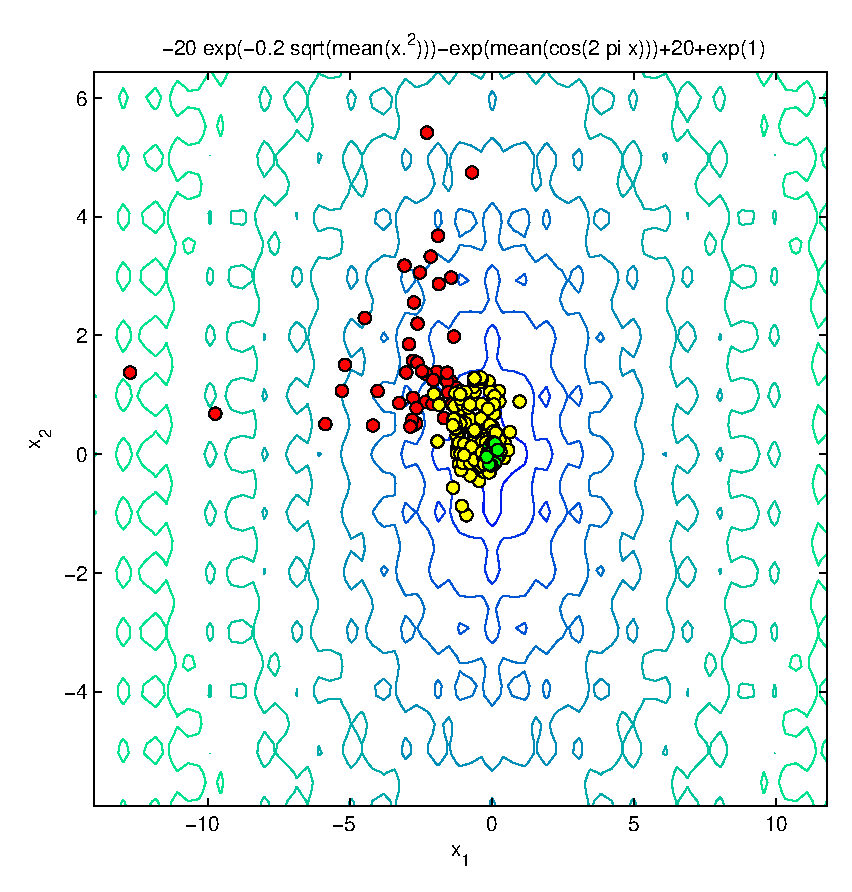
\includegraphics[scale=0.55]{ES_ackley_curvNivel.eps}
\caption{Função Ackley minimizada com Estratégias Evolutivas - Curva de Nível e indivíduos das populações}
\label{fig:ES_ackley_curvNivel}
\end{figure}

Testou-se também a aplicação do algoritmo à mesma função Ackley com três dimensões. Desta vez, utilizou-se um tamanho de população de  $\mu=70$ e $\lambda=300$ filhos.

Ademais, escolheu-se $\varepsilon_a=10^{-10}$ e $\varepsilon_r=10^{-10}$ para o critério de parada, bem como $\varepsilon=10^{-2}$, $\alpha_1=\alpha_2=1$ como parâmetros de mutação. A condição inicial aqui foi $x_0 = \begin{bmatrix}2 &1&0.5\end{bmatrix}.$

O minimizador indicado pelo algoritmo nesse caso foi $x= \begin{bmatrix}0.0000&0.0219&0.0512\end{bmatrix}^T$, ponto cuja avaliação da função foi 0.1827, encontrado em duas gerações de população, conforme a tabela da figura \ref{fig:table3dim}.

\begin{table}[!htcb]
  \centering
  \begin{tabular}{|c|c|c|c|c|}
    \hline
    \rowcolor{kugray5}
    &    $x(1)$   &    $x(2)$   &    $x(3)$    &   $f(x)$  \\ \hline
	\cellcolor{kugray5}1   &   0.8768   &     0.7696	&    0.2084    &   3.8348  \\ \hline	
    \rowcolor{kugray5}
		2   &   0.8333   &    -0.1687	&    0.2802    &   3.3766  \\ \hline
	\cellcolor{kugray5}3   &   -0.0000   &    0.0219	&    0.0512    &   0.1827  \\ \hline
	\end{tabular}
  \caption{Tabela com os melhores indivíduos de cada geração e o valor da função objetivo avaliada - caso 3 dimensões}
  \label{fig:table3dim}
\end{table}

A figura \ref{fig:ES_ackley_3dim} mostra graficamente o resultado desta tabela, apresentando o valor da função objetivo avaliada no indivíduo mais apto da população de cada geração.

\begin{figure}[!htcb]
\centering
\includegraphics[scale=0.45]{ES_ackley_3dim.eps}
\caption{Evolução da Função Ackley avaliada para o melhor indivíduo da população em cada geração- caso 3 dimensões}
\label{fig:ES_ackley_3dim}
\end{figure}

\section{Conclusões}

Conclui-se que ambos os algoritmos apresentaram excelentes performances no que se refere à minimização de funções complexas, com diversos mínimos locais e mesmo com dimensões elevadas do problema. 

Inclusive, em comparação com os métodos determinísticos que haviam sido estudados até então, os métodos estocásticos parecem ser boas alternativas para evitar que o algoritmo de otimização escolhido fique retido em mínimos locais.

No entanto, é importante frisar a natureza estocástica dos métodos apresentados neste relatório. Portanto, mesmo se exatamente os mesmos parâmetros forem inicializados, o comportamento do processo pode ser diferente a cada rodada.

Neste relatório, foram apresentados os resultados de uma única rodada. Entretanto, a indicação normalmente para esses métodos estocásticos é a de que se rode o algoritmo outras vezes e se obtenha uma média dos resultados para maior robustez.

\begin{thebibliography}{1}

\bibitem{notas_aula_JG}
José Gabriel R.C.Gomes, Notas de aula CPE723 Otimização Natural,COPPE.

\bibitem{SA}
S. Kirkpatrick, C. D. Gelatt Jr., e M. P. Vecchi. Optimization by simulated annealing. Science, vol. 220, pp.
671-680, maio de 1983.

\bibitem{FSA}
H. Szu e R. Hartley. Fast simulated annealing. Physics Letters A, vol. 122, no. 3-4, pp. 157-162, junho de
1987.

\bibitem{livro_AG}
A. E. Eiben e J. E. Smith. Introduction to Evolutionary Computing. Ed. Springer, 2007 (2003). ISSN
1619-7127.

\bibitem{metropolis}
N. Metropolis, A. W. Rosenbluth, M. N. Rosenbluth, A. H. Teller, e E. Teller. Equation of state calculation by fast computing machines. The Journal of Chemical Physics, vol. 21, no. 6, pp. 1087-1092, junho de 1953.

\end{thebibliography}


\end{document}

